\newpage
\section{Image processing}

There is several way for embedded image processing on linux board. The first one studied in assignment 7 and 8 is gstreamer librairies. This librairies allow us to build a so called pipeline that take picture from camera and is able to expose each sample for processing or save them. There is no direct image processing functions and we have to create our own or link to an other librairie. An alternative to gstreamer is ffmpeg. Ffmpeg also allows us to build pipeline for capturing video from a webcam. Ffmpeg has more filter and functions than gstreamer but don't have an as good API for extending it. There is a third solution which is opencv. Opencv is the reference in term of open-source image processing. It can be link to both gstreamer and ffmpeg and even work alone. Because it's processing oriented, it will have less options for capturing data. 

\subsection{Gstreamer }

Because of assignment 7 and 8 ask to build a processing chain with gstreamer, we first tried to use it for image processing. The idea was that we already have a working chain and image detection didn't need to be so accurate so we should be able to create our own detecting algorithm and get satisfying results.

\subsubsection{Pipeline Gstreamer}
The first step already done with assignement 7 and  8 was to setup a pipeline that get the video and separate each frame for processing. 

\begin{figure}[!ht]
\centering
 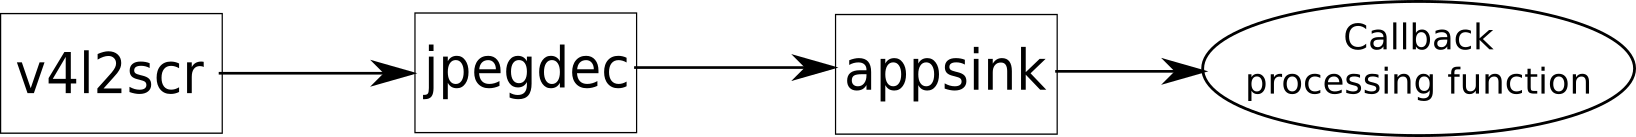
\includegraphics[width=0.7\textwidth]{gst_pipeline.png}
 \caption{Gstreamer pipeline for image processing}
 \label{gst_pip}
\end{figure}

\subsubsection{Image processing}

The algorithm for image processing was first an obvious one. The idea was to detect a rectangle of a particular color. We checked each pixel and if there is enough pixel with the right value following in the same line, we go to next line until we have enough line to say that we found the shape.

\begin{figure}[!ht]
\centering
 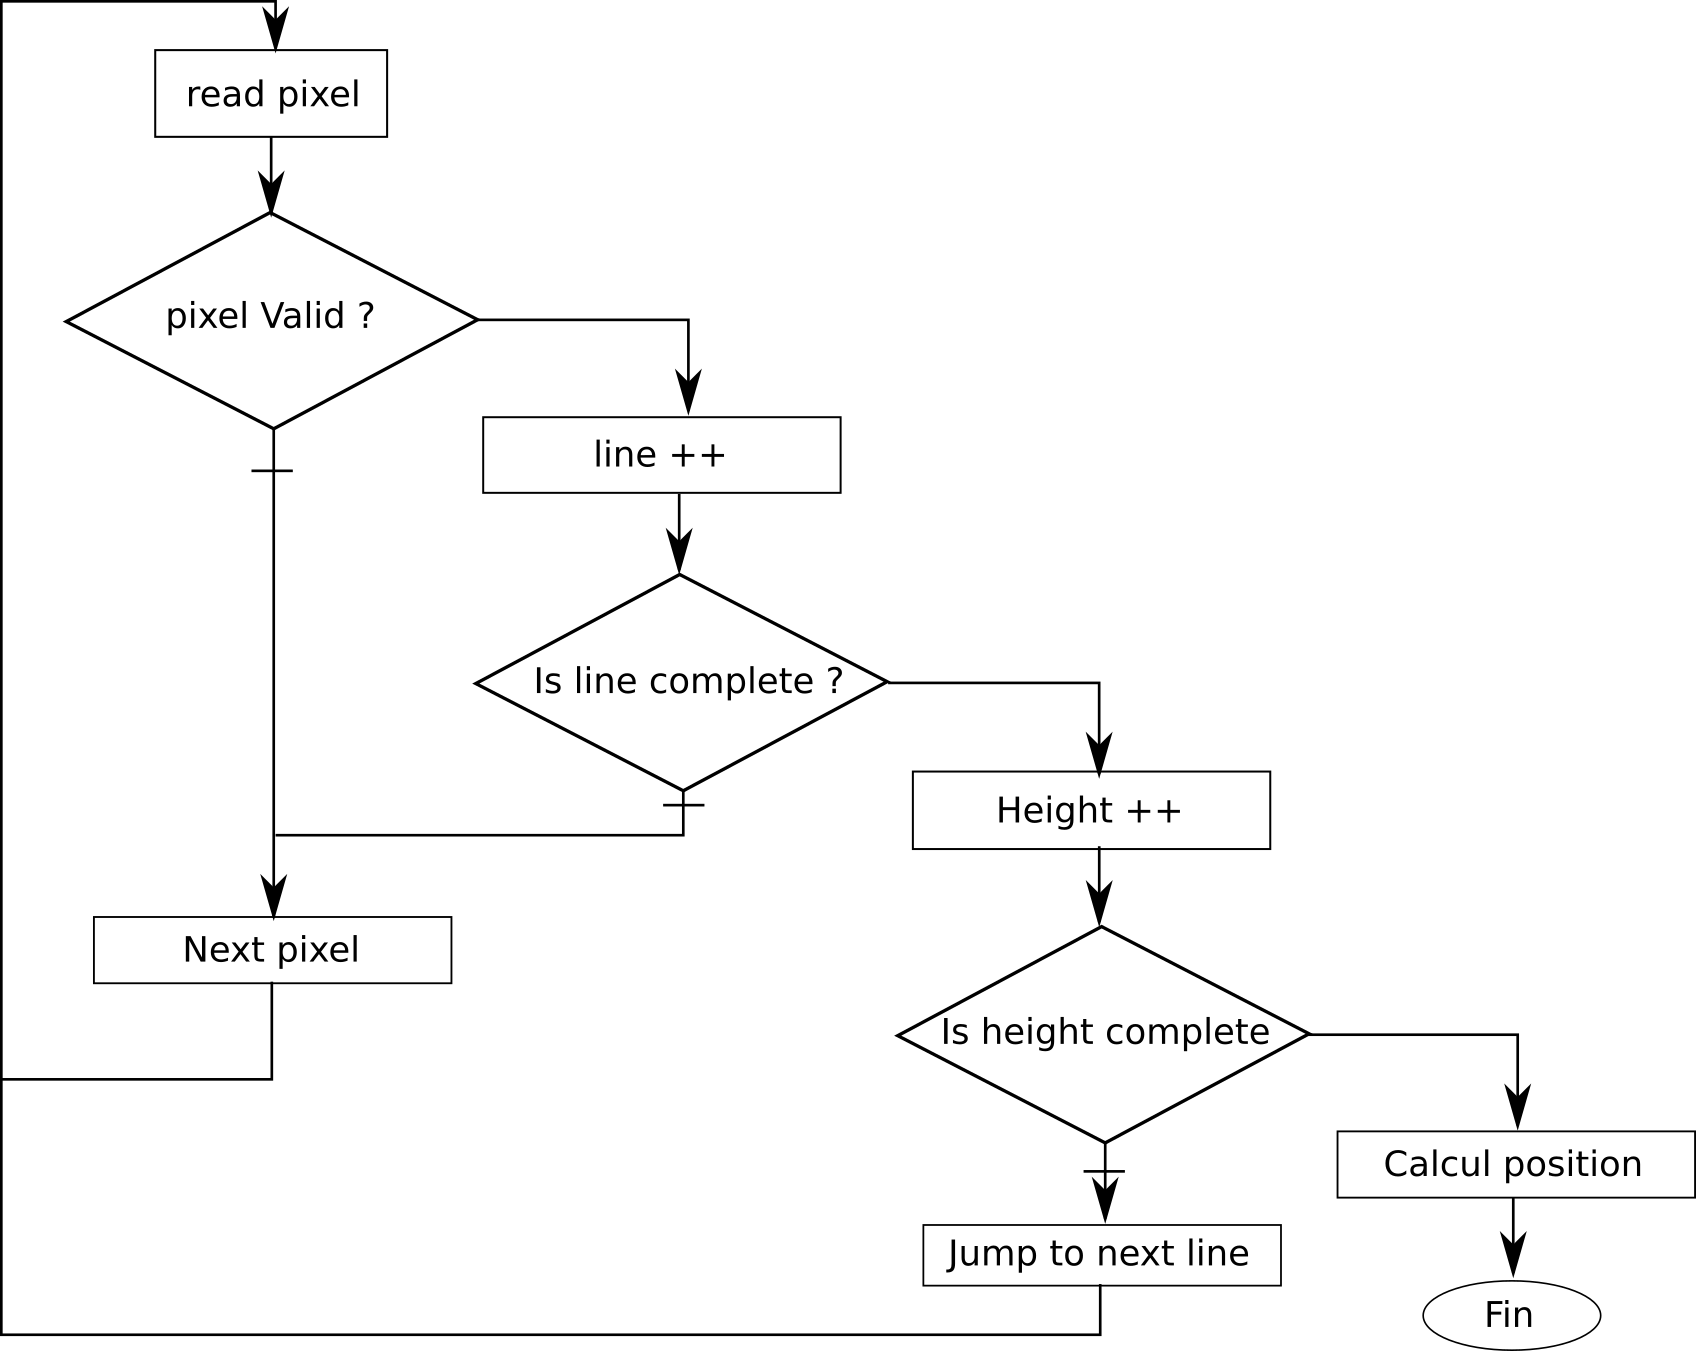
\includegraphics[width=0.7\textwidth]{detection_algo.png}
 \caption{Shape detection algorithm}
 \label{spe_det}
\end{figure}

After some tests, this algorithm was not efficient enough so we did some improvements : 

\begin{itemize}
 \item \textbf{Wrong pixel tolerance : } we accepted that a part of the pixel could not valid the threshold
 \item \textbf{Variable size : } Our first try used a fixe size for the shape. The center point found was so not well placed.
\end{itemize}

\subsubsection{Results}

Despite the improvement of the algorithm, the results where still not accurate enough. To get more precision, we did a test. We captured  some pictureform the camera with the shape. After that, we modified each picture in order to have the shape at a specific place, combined it into a video and then we tested our algorithm on it. We got the following results : 

    \begin{center}
\begin{tabular}{|c|c|c|}\hline
Algorithm result (px) & real result (px) & Error (\%)\\\hline
nothing & 20x20 & n.a.\\\hline
64x35 & 60x20 & 2,5x12,5\\\hline
75x15 & 100x20 & 15,6x4,2\\\hline
150x23 & 140x20 & 6,25x2,5\\\hline
32x41 & 20x60 & 7,5x15,8\\\hline
54x86 & 60x60 & 3,72x21,7\\\hline
102x54 & 100x60 & 1,25x5\\\hline
120x57 & 140x60 & 12,5x2,5\\\hline
10x86 & 20x100 & 6,25x11,6\\\hline
53x100 & 60x100 & 4,375x0\\\hline
93x120 & 100x100 & 4,75x16,7\\\hline
124x106 & 140x100 & 10x5\\\hline
    \end{tabular}
    \end{center}

Has we can see, the incertitude is really high so we cannot really use it.

\subsection{Opencv}

Because of implementing an algorithm by ourselves was not accurate enough, we decided so to use opencv librairy. As explain before, opencv is one of the most used librairy for image processing and there is already a lot of examples that are almost altready working. We get an algorithm that find all the pixel in a spécific range of value and then calculate the moment of all of them in order to find the center. This algorithm add also some mecanism for filtering alone pixels in order to reduce false positive pixels.
.

